In diesem Abschnitt werden die allgemeine Informationen von FastTrack dargestellt.
Dann wird Teil \ref{subsec:netAuf} der Allgemeine Aufbau des Netzwerkes dargestellt. 
Im Unterabschnitt \ref{subsec:proAuf} wird der Aufbau des Programm eines Knoten beschrieben.
Der Aufbau des Netzwerkes und des Knoten Programms wurde aus dem Artikel \cite{liang2006fasttrack} genommen.

\subsection{Netzwerk Aufbau}
\label{subsec:netAuf}

Das Netzwerk besteht aus Knoten die untereinander verbunden sind.
Diese unterteilen sich in normale Knoten (ON) und Superknoten (SN).
Es ist ähnlich der Abbildung \ref{fig:auf} aufgebaut.
Die ONs sind mit jeweils einen SN verbunden, welchen sie nach dem Betreten des Netzwerk wählen.
Die SNs speichern dabei die Metainformationen seiner Knoten.
Diese werden bei einer Suchanfrage der Knoten durchsucht durchsucht.
Außerdem sind die SNs untereinander verbunden um Informationen auszutauschen und Suchanfragen weiterzuleiten.

\begin{figure}
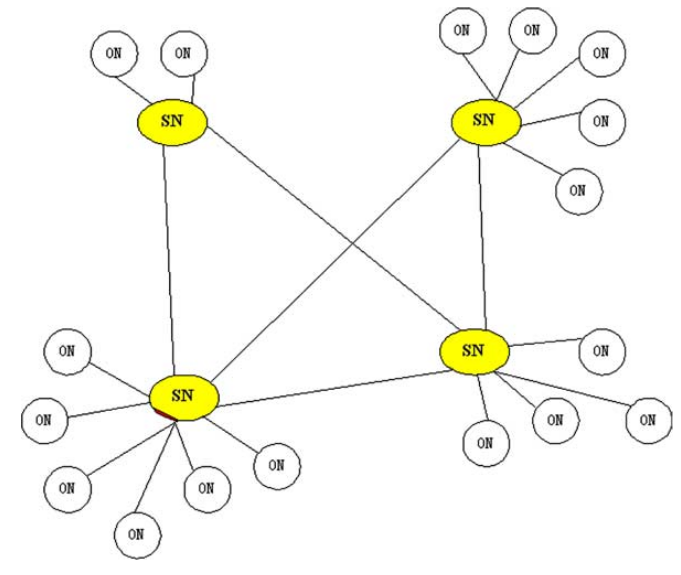
\includegraphics[scale=0.3]{gfx/aufbau}
\caption{Aufbau des FastTrack Netzwerkes (Quelle \cite{liang2006fasttrack})}
\label{fig:auf}
\end{figure}

\subsubsection{Superknoten}

Jeder Knoten im Netzwerk, kann ein SN werden.
Die Wahl ob ein Knoten ein SN wird dabei beachtet wie die Knoten an  das Internet angebunden ist und wie leistungsstark der Knoten ist.
Es ist wichtig, dass die Verbindung zum Internet schnell genug ist, da häufig Anfragen an die SN kommen können.
Außerdem damit die Verarbeitung der Anfrage schnell gehen, sollte auch die Hardware  entsprechende Leistung besitzen.

\subsection{Knoten Programm Aufbau}
\label{subsec:proAuf}

Die offiziellen Klienten \textit{Kazaa}\cite{kazaa} sind nur für Windows vorhanden
Er besteht aus vier Komponenten, die folgend vorgestellt werden:

\begin{itemize}
\item[1.] \textbf{GUI:} Die GUI des Windows Klienten für die Eingab von Suchanfragen und anzeigen der Downloads.
\item[2.] \textbf{Windows Register:} In der Windows Registry ist der Cache der SuperKnoten gespeichert.
Dieser enthält für jeden Knoten die IP, den Port, die Auslastung und einen Zeitangabe, wann die Information das letzte mal aktualisiert wurden.
\item[3.] \textbf{DDB Dateien:} In den DDB Dateien sind die Metainformation der eigenen Dateien gespeichert. Es wird der Name, die Größe, der ContentHash und die Beschreibung der Daten. Diese werden zum Beispiel für die Suche verwendet, wenn die Metadaten zum SN gesendet werden.
\item[4.] \textbf{DAT-Dateien:} Diese Dateien enthalten die heruntergeladenen Daten, welche am Ende umbenannt werden.
\end{itemize}

